\documentclass[xetex,10pt,dvipsnames,svgnames]{beamer}

%% standard packages
\usepackage{mathpartir}
\usepackage{amsmath}
\usepackage{amssymb}
\usepackage{stmaryrd}

\usetheme{metropolis}

%% font/input settings
\usepackage[english]{babel}
\usepackage{fontawesome}

\usepackage{tikz}
\usetikzlibrary{matrix,
  positioning,
  backgrounds,
  shapes,
  shapes.callouts,
  automata,
  fit,
  decorations.pathreplacing,
  patterns
}

\tikzstyle{every picture}+=[remember picture]

%% Andreas' isa constant package
% Author: Andreas Lochbihler, ETH Zurich
% Version 0.2 (2014-11-19)

\makeatletter
% \newcommand{\gobble}{\@gobble}

%Umsetzung von lateinischen Kleinbuchstaben in griechische:
\def\greek@a{\alpha}
\def\greek@b{\beta}
\def\greek@c{\chi}
\def\greek@d{\delta}
\def\greek@e{\varepsilon}
\def\greek@f{\varphi}
\def\greek@g{\gamma}
\def\greek@h{\eta}
\def\greek@i{\iota}
\def\greek@k{\kappa}
\def\greek@l{\lambda}
\def\greek@m{\mu}
\def\greek@n{\nu}
\def\greek@o{\omicron}
\def\greek@p{\pi}
\def\greek@q{\theta}
\def\greek@r{\rho}
\def\greek@s{\sigma}
\def\greek@t{\tau}
\def\greek@u{\upsilon}
\def\greek@w{\omega}
\def\greek@x{\xi}
\def\greek@y{\psi}
\def\greek@z{\zeta}
\def\make@greek#1{\csname greek@#1\endcsname}
\def\@allgreek#1#2\@stopallgreek{%
  \make@greek{#1}%
  \def\@testa{}\def\@testb{#2}%
  \ifx\@testa\@testb\relax\else\@allgreek #2\@stopallgreek\fi
}
\newcommand{\greek}[1]{%
  \def\@testa{}\def\@testb{#1}
  \ifx\@testa\@testb\relax\else\@allgreek #1\@stopallgreek\fi%
}

% Formatierung fuer Formel-Konstanten
% funktioniert auch mit Hoch-/Tiefstellung, Schriftgroesse des Kontexts wird uebernommen,
% Vorschub ist 10% groesser als Schriftgroesse
\newlength{\isa@vorschub}
\ifx\beamer@version\relax
  \newcommand{\@innersyntax}[2]{%
    \def\@tempa##1{%
      \setlength{\isa@vorschub}{##1pt}%
      \mathord{\emph{\text{\fontsize{##1}{1.1\isa@vorschub}\selectfont#1#2}}}%
    }%
    \mathchoice%
      {\@tempa{\tf@size}}%
      {\@tempa{\tf@size}}%
      {\@tempa{\sf@size}}%
      {\@tempa{\ssf@size}}%
  }%
\else
  \newcommand{\@innersyntax}[2]{%
    \def\@tempa##1{%
      \setlength{\isa@vorschub}{##1pt}%
      \mathord{\text{\fontsize{##1}{1.1\isa@vorschub}\selectfont#1#2}}%
    }%
    \mathchoice%
      {\@tempa{\tf@size}}%
      {\@tempa{\tf@size}}%
      {\@tempa{\sf@size}}%
      {\@tempa{\ssf@size}}%
  }%
\fi
\newcommand{\isaconst}[1]{\textsf{\textup{#1}}}
\newcommand{\isatype}[1]{\textsf{\textup{#1}}}
\newcommand{\isacommand}[1]{\textrm{\bfseries #1}}
\newcommand{\isaminorkeyword}[1]{\textrm{#1}}
\newcommand{\isaprooftemplate}{\langle\!\langle\mathord{\text{proof}}\rangle\!\rangle}
\newcommand{\isanameprefix}[1]{\textit{#1}}
\newcommand{\isamethod}[1]{\textrm{#1}}

\def\DeclareIsaConst{\@star@or@long\Decl@reIs@Const}
\def\Decl@reIs@Const#1{%
  \expandafter\@testopt%
    \expandafter{%
    \expandafter\@newcommand%
    \expandafter{%
      \csname isa:const:#1\endcsname%
    }%
  }0%
}

\def\DeclareIsaType{\@star@or@long\Decl@reIs@Type}
\def\Decl@reIs@Type#1{%
  \expandafter\@testopt%
    \expandafter{%
    \expandafter\@newcommand%
    \expandafter{%
      \csname isa:type:#1\endcsname%
    }%
  }0%
}

\def\DeclareIs@Index#1#2#3#4#5{
  \def\testa{}\def\testb{#5}%
  \ifx\testa\testb
    \expandafter\newcommand%
    \csname isa:#1:#2\endcsname[1][]%
    {%
      \def\testa{}\def\testb{##1}\def\testc{(}\def\testd{)}%
      \ifx\testa\testb
        \index{#3@\isa{#4}}%
      \else\ifx\testb\testc
        \index{#3@\isa{#4}|(}%
      \else\ifx\testb\testd
        \index{#3@\isa{#4}|)}%
      \else
        \index{#3@\isa{#4}!##1}%
      \fi\fi\fi
    }%
  \else
    \expandafter\newcommand%
    \csname isa:#1:#2\endcsname[1][]%
    {%
      \def\testa{}\def\testb{##1}\def\testc{(}\def\testd{)}%
      \ifx\testa\testb
        \index{#3@\isa{#4}\indexxpl{#5}}%
      \else\ifx\testb\testc
        \index{#3@\isa{#4}\indexxpl{#5}|(}%
      \else\ifx\testb\testd
        \index{#3@\isa{#4}\indexxpl{#5}|)}%
      \else
        \index{#3@\isa{#4}\indexxpl{#5}!##1}%
      \fi\fi\fi
    }
  \fi
}

\def\DeclareIs@IndexSub#1#2#3#4#5{
  \expandafter\newcommand%
  \csname isa:#1:#2\endcsname[1][]%
  {%
    \def\testa{}\def\testb{##1}\def\testc{(}\def\testd{)}%
    \ifx\testa\testb
      \index{#3@\isa{#4}!#5}%
    \else\ifx\testb\testc
      \index{#3@\isa{#4}!#5|(}%
    \else\ifx\testb\testd
      \index{#3@\isa{#4}!#5|)}%
    \else
      \index{#3@\isa{#4}!#5!##1}%
    \fi\fi\fi
  }%
}

\def\DeclareIsaIndexTN{\DeclareIs@Index{indext}}
\def\DeclareIsaIndexTS{\DeclareIs@IndexSub{indext}}
\def\DeclareIsaIndexCN{\DeclareIs@Index{indexc}}
\def\DeclareIsaIndexCS{\DeclareIs@IndexSub{indexc}}

\newcommand{\DeclareIsaIndexT}{\@ifstar\DeclareIsaIndexTS\DeclareIsaIndexTN}
\newcommand{\DeclareIsaIndexC}{\@ifstar\DeclareIsaIndexCS\DeclareIsaIndexCN}

\DeclareRobustCommand{\isa}[1]{\bgroup\activateisacommands \ensuremath{#1}\egroup}
\def\inner@synt@x#1#2{%
  \expandafter\ifx\csname isa:#1:#2\endcsname\relax%
    \relax \@latex@error{Isabelle #1 #2 undefined}\@ehc%
  \else%
    \def\@tempa{\csname isa:#1:#2\endcsname}%
    \expandafter\@tempa%
  \fi%
}
\newcommand{\activateisacommands}{%
  \def\c{\inner@synt@x{const}}%
  \def\t{\inner@synt@x{type}}%
  \def\tv##1{\greek{##1}}%
  \def\hastype{\mathrel{::}}%
  \def\hassort{\mathrel{::}}%
  \def\command{\isacommand}%
  \def\minorkeyword{\isaminorkeyword}%
  \def\prooftemplate{\isaprooftemplate}%
  \def\nameprefix{\isanameprefix}%
  \def\llistOf{\overline}%
  \def\listOf{\underline}%
}
\newcommand{\isaindexc}{\inner@synt@x{indexc}}
\newcommand{\isaindext}{\inner@synt@x{indext}}
\makeatother

% Reference Isabelle theorems in LaTeX text by name without printing
\newcommand{\refthm}[1]{}

\newcommand{\isaunderscore}{\mbox{-}}

% Koinduktive Regeln mit doppelter Linie
\makeatletter
\newlength\conclusion@length
\newcommand{\oldcoinferrule}[2]{%
  \def\@premise{#1}%
  \def\@conclusion{\ensuremath{#2}}%
  \def\@testb{ }%
  \ifx\@premise\@testb%
    \relax
    \settowidth\conclusion@length{\@conclusion}%
    \def\@premise{\rule{\conclusion@length}{0cm}}%
  \fi%
  \ensuremath{{\mprset{fraction={===}}\inferrule{\@premise}{\@conclusion}}}%
}
\makeatother

\makeatletter
\newlength{\extrarowsep}
\setlength{\extrarowsep}{1.8ex}
\newcommand{\rowsep}{%
  \noalign{\ifnum0=`}\fi
  \@ifnextchar[{\@rowsep}{\@rowsep[\extrarowsep]}%
}
\def\@rowsep[#1]{%
  \hrule height #1 width 0cm \relax \ifnum0=`{\fi}%
}
\makeatother

% Tabelle fuer inferrules, die zweite Spalte fuer die Regeln nimmt so viel Platz wie moeglich,
% weniger dem Platz der ersten Spalte
\newlength{\formulacolumnwidth}%
\newenvironment{inferruletable}[1][\linewidth]{%
  % X-Spalte zentriert setzen
  \renewcommand{\tabularxcolumn}[1]{>{\setlength{\formulacolumnwidth}{##1}}c}%
  \let\oldinferrule=\inferrule%
  \let\oldcoinferrule=\coinferrule%
  \renewcommand{\inferrule}[2]{\ensuremath{\hsize=\formulacolumnwidth\oldinferrule{##1}{##2}}}%
  \renewcommand{\coinferrule}[2]{\ensuremath{\hsize=\formulacolumnwidth\oldcoinferrule{##1}{##2}}}%
  \tabularx{#1}{@{}l@{~}X@{}}%
}{
  \endtabularx%
}



\makeatletter
\def\@gatherrulesand{%
  \ifmmode $ \fi%
  \hskip 2em plus 0.5fil minus 0.5em%
  $%
}
\def\gatherrules@bindings{%
  \let\par\@gatherrulesand%
}
\newenvironment{gatherrules}{%
  \trivlist \centering \item\relax 
  \lineskiplimit=1.2em\lineskip=1.2em plus 0.2em%
  \bgroup%
  \gatherrules@bindings%
  \protect\centering%
  $%
}{$\egroup \endtrivlist}
\makeatother

\colorlet{greybackground}{black!25}
\colorlet{greyforeground}{black!50}
\newcommand{\highlight}[1]{\colorbox{greybackground}{$\!#1\!$}}
\newcommand{\highlightsmash}[1]{\vphantom{Ag}\smash{\highlight{\vphantom{X}\smash{#1}}}}

\newlength{\spacewidth}
\newcommand{\halfspace}{\settowidth{\spacewidth}{\ }\relax\hspace{0.5\spacewidth}}

\newcommand{\programfont}{\tt}
\newcommand{\programtext}[1]{\texttt{#1}}

\newcommand{\marknewfeature}{$\ast$}


% Isabelle library types
% ======================
\DeclareIsaType{_}{\_}
\DeclareIsaType{unit}{\isatype{unit}}
\DeclareIsaType{nat}{\isatype{nat}}
\DeclareIsaType{bool}{\isatype{bool}}
\DeclareIsaType{int}{\isatype{int}}
\DeclareIsaType{rat}{\isatype{rat}}
\DeclareIsaType{real}{\isatype{real}}
\DeclareIsaType{fun}[2]{#1 \mathbin{\Rightarrow} #2}
\DeclareIsaType{=>}{\mathbin{\Rightarrow}}
\DeclareIsaType{prod}[2]{#1 \mathbin{\times} #2}
\DeclareIsaType{*}{\mathbin{\times}}
\DeclareIsaType{sum}[2]{#1 \mathbin{+} #2}
\DeclareIsaType{+}{\mathbin{+}}
\DeclareIsaType{option}[1]{#1\ \isatype{option}}
\DeclareIsaType{list}[1]{#1\ \isatype{list}}
\DeclareIsaType{array}[1]{#1\ \isatype{array}}
\DeclareIsaType{filter}[1]{#1\ \isatype{filter}}
\DeclareIsaType{set}[1]{#1\ \isatype{set}}
\DeclareIsaType{ennreal}{\overline{\mathbb{R}}_{\ge 0}}

\DeclareIsaType{completelattice}{\isatype{complete}\isaunderscore \isatype{lattice}}
\DeclareIsaType{completelinorder}{\isatype{complete}\isaunderscore \isatype{linorder}}
\DeclareIsaType{topologicalspace}{\isatype{topological}\isaunderscore \isatype{space}}

% Isabelle library constant
% =========================
\DeclareIsaConst{[|}{\llbracket}
\DeclareIsaConst{|]}{\rrbracket}
\DeclareIsaConst{==>}{\Longrightarrow}

\DeclareIsaConst{==}{\equiv}

\DeclareIsaConst{op}[1]{\isaconst{op}\ \mathord{#1}}

\DeclareIsaConst{->}{\to}
\DeclareIsaConst{_}{\_}
\DeclareIsaConst{_case_case}{\isaconst{case}}
\DeclareIsaConst{_case_of}{\isaconst{of}}
\DeclareIsaConst{_case_=>}{\mathrel{\Rightarrow}}
\DeclareIsaConst{_case_|}{\mathrel{|}}
\DeclareIsaConst{_let_let}{\isaconst{let}}
\DeclareIsaConst{_let_in}{\isaconst{in}}
\DeclareIsaConst{id}{\isaconst{id}}
\DeclareIsaConst{-->}{\longrightarrow}
\DeclareIsaConst{and}{\mathrel{\wedge}}
\DeclareIsaConst{or}{\mathrel{\vee}}
\DeclareIsaConst{<-->}{\longleftrightarrow}
\DeclareIsaConst{undefined}{\isaconst{undefined}}
\DeclareIsaConst{if}{\mathrel{\isaconst{if}}}
\DeclareIsaConst{then}{\mathrel{\isaconst{then}}}
\DeclareIsaConst{else}{\mathrel{\isaconst{else}}}
\DeclareIsaConst{()}{\mathord{(}\mathord{)}}
\DeclareIsaConst{in}{\mathrel{\isaconst{in}}}
% \DeclareIsaConst{funpow}{\mathrel{\textrm{\textasciicircum\textasciicircum}}}
\DeclareIsaConst{DUMMY}{\mathrel{\isaunderscore}}

\DeclareIsaConst{True}{\isaconst{True}}
\DeclareIsaConst{False}{\isaconst{False}}
\DeclareIsaConst{Not}{\isaconst{Not}}

\DeclareIsaConst{fst}{\isaconst{fst}}
\DeclareIsaConst{snd}{\isaconst{snd}}
\DeclareIsaConst{Inl}{\isaconst{Inl}}
\DeclareIsaConst{Inr}{\isaconst{Inr}}


\DeclareIsaConst{THE}[2]{\iota#1.\,#2}
\DeclareIsaConst{_THE}{\iota}
\DeclareIsaConst{_Eps}{\varepsilon}
\DeclareIsaConst{SOME}[2]{\c{_Eps}#1.\ #2}
\DeclareIsaConst{LEAST}[2]{\isaconst{LEAST}\ #1.\ #2}
\DeclareIsaConst{_LEAST}{\isaconst{LEAST}}

\DeclareIsaConst{uminus}{\mathord{-}}
\DeclareIsaConst{Set.uminus}[1]{\mathord-\,#1}


\DeclareIsaConst{None}{\isaconst{None}}
\DeclareIsaConst{Some}[1][]{%
  \def\testa{#1}\def\testb{}%
  \ifx\testa\testb\isaconst{Some}\else\mathord\lfloor#1\mathord\rfloor\fi%
}
\DeclareIsaConst{SomeL}{\mathord\lfloor}
\DeclareIsaConst{SomeR}{\mathord\rfloor}
\DeclareIsaConst{the}{\isaconst{the}}
\DeclareIsaConst{_option_case}[4]{\c{_case_case}\ #1\ \c{_case_of}\ \c{None} \c{_case_=>} #2\ |\ \c{Some}[#3] \c{_case_=>} #4}
\DeclareIsaConst{Option.map}{\isaconst{Option.map}}


\DeclareIsaConst{Set.empty}{\emptyset}
\DeclareIsaConst{insert}{\isaconst{insert}}
\DeclareIsaConst{UNIV}{\isaconst{UNIV}}
\DeclareIsaConst{image}[2]{#1 \mathbin{`} #2}
\DeclareIsaConst{finite}{\isaconst{finite}}
\DeclareIsaConst{infinite}{\isaconst{infinite}}

\DeclareIsaConst{singleton}[1]{\{\,#1\,\}}
\DeclareIsaConst{Un}{\mathrel{\cup}}
\DeclareIsaConst{Int}{\mathrel{\cap}}
\DeclareIsaConst{Union}[1]{\bigcup #1}
\DeclareIsaConst{UN}[2]{\bigcup_{#1} #2}
\DeclareIsaConst{Inter}[1]{\bigcap #1}
\DeclareIsaConst{INT}[2]{\bigcap_{#1} #2}
\DeclareIsaConst{<+>}{\uplus}
\DeclareIsaConst{Pow}[1]{\mathcal{P}(#1)}
\DeclareIsaConst{range}{\isaconst{range}}
\DeclareIsaConst{restrictrelation}[2]{\mathrel{\left.\mathord{#1}\right|_{#2}}}
\DeclareIsaConst{inv_imageP}[2]{#2^{-1}(#1)}
\DeclareIsaConst{:}{\in}
\DeclareIsaConst{/:}{\notin}
\DeclareIsaConst{card}[1]{||#1||}
\DeclareIsaConst{bind}{\isaconst{bind}}
\DeclareIsaConst{bind*}{\mathrel{>\!\!>\!\!=}}
\DeclareIsaConst{return}{\isaconst{return}}
\DeclareIsaConst{::}{::}

\DeclareIsaConst{lfp}{\isaconst{lfp}}
\DeclareIsaConst{gfp}{\isaconst{gfp}}

\DeclareIsaConst{SUP}[2]{\bigsqcup_{#1} #2}
\DeclareIsaConst{INF}[2]{\bigsqcap_{#1} #2}

\DeclareIsaConst{inj_on}{\isaconst{inj\isaunderscore on}}

\DeclareIsaConst{Min}{\isaconst{Min}}

\DeclareIsaConst{div}{\mathbin{\isaconst{div}}}
\DeclareIsaConst{int}{\isaconst{int}}
\DeclareIsaConst{nat}{\isaconst{nat}}
\DeclareIsaConst{>=}{\ge}
\DeclareIsaConst{<}{<}
\DeclareIsaConst{>}{>}
\DeclareIsaConst{op >}{\isaconst{op}\ \mathord{>}}
% \DeclareIsaConst{Suc}{\isaconst{Suc}}
\DeclareIsaConst{max}{\isaconst{max}}

\newcommand{\lub}{\mathord{\textstyle\bigvee}}


\DeclareIsaType{enat}{\isatype{enat}}

\DeclareIsaConst{enat_unfold}{\isaconst{enat\isaunderscore unfold}}
% \DeclareIsaConst{eSuc}{\isaconst{eSuc}}
\DeclareIsaConst{infinity}{\infty}
\DeclareIsaConst{the_enat}{\isaconst{nat\isaunderscore of}}

\DeclareIsaType{ereal}{\isatype{ereal}}

\DeclareIsaType{measure}[1]{#1\ \isatype{measure}}
\DeclareIsaConst{space}{\isaconst{space}}
\DeclareIsaConst{sets}{\isaconst{sets}}
\DeclareIsaConst{emeasure}{\isaconst{emeasure}}
\DeclareIsaConst{measure}{\isaconst{measure}}
\DeclareIsaConst{nnint}[2]{\int #1~\isaconst{d}#2}
\DeclareIsaConst{nnint*}[3]{\int_#2 #2~\isaconst{d}#3}
\DeclareIsaConst{integrable}{\isaconst{integrable}}
\DeclareIsaConst{sfmeasure}{\isaconst{sigma\isaunderscore finite\isaunderscore measure}}

\DeclareIsaConst{density}{\isaconst{density}}
\DeclareIsaConst{distr}{\isaconst{distr}}
\DeclareIsaConst{uniform}{\isaconst{cprob}}
\DeclareIsaConst{count}{\isaconst{count\isaunderscore space}}
\DeclareIsaConst{point}{\isaconst{point\isaunderscore measure}}

\DeclareIsaConst{salgebra}{\isaconst{sigma\isaunderscore algebra}}
\DeclareIsaConst{measurespace}{\isaconst{measure\isaunderscore space}}
\DeclareIsaConst{Nat}{\mathbb{N}}
\DeclareIsaConst{measurable}[2]{#1 \to^{\!\sigma} #2}
% \DeclareIsaConst{Measurable.pred}[2]{\isaconst{Measurable.pred}\ #1\ #2}
\DeclareIsaConst{bool}{\isaconst{bool}}
\DeclareIsaConst{restrict}{\isaconst{restrict\isaunderscore space}}
\DeclareIsaConst{vsigma}{\isaconst{vsigma}}
\DeclareIsaConst{sigma}{\isaconst{sigma}}
\DeclareIsaConst{Supsigma}{{\textstyle \bigsqcup^{\sigma}}}
\DeclareIsaConst{SUPsigma}[2]{\mathop{{\bigsqcup}^{\sigma}\kern-1.3ex}_{#1} #2}
\DeclareIsaConst{prodM}[2]{#1\ {\times^\sigma}\ #2}
\DeclareIsaConst{ProdM}[2]{\mathop{{\prod}^{\sigma}\kern-1.3ex}_{#1}\ #2}
\DeclareIsaConst{pred}{\isaconst{pred}}
\DeclareIsaConst{indicator}{\isaconst{indicator}}
\DeclareIsaConst{AE}[3]{A\!E~#1~\isaconst{in}~#2.~#3}
\DeclareIsaConst{prob}[3]{\Pr\left(#1 ~\isaconst{in}~#2.~#3\right)}
\DeclareIsaConst{cprob}[4]{\Pr\left(#1 ~\isaconst{in}~#2.~#3~|~#4\right)}

\DeclareIsaConst{mono}{\isaconst{mono}}
\DeclareIsaConst{antimono}{\isaconst{antimono}}
\DeclareIsaConst{probspace}{\isaconst{prob\isaunderscore space}}
\DeclareIsaConst{subprobalgebra}{\isaconst{subprob\isaunderscore algebra}}
\DeclareIsaConst{subprob}{\isaconst{subprob}}
\DeclareIsaConst{borel}{\isaconst{borel}}
\DeclareIsaConst{lborel}{\isaconst{lborel}}
\DeclareIsaConst{open}{\isaconst{open}}
\DeclareIsaConst{continuouson}{\isaconst{continuous\isaunderscore on}}
\DeclareIsaConst{supcontinuous}{\sqcup{-}\isaconst{continuous}}
\DeclareIsaConst{infcontinuous}{\isaconst{inf\isaunderscore continuous}}
\DeclareIsaConst{countable}{\isaconst{countable}}


\DeclareIsaConst{streamspace}{\isaconst{stream\isaunderscore space}}

\DeclareIsaType{pmf}[1]{#1\ \isaconst{pmf}}
\DeclareIsaConst{measurepmf}{\isaconst{measure\isaunderscore pmf}}
\DeclareIsaConst{bindpmf}{\isaconst{bind\isaunderscore pmf}}
\DeclareIsaConst{returnpmf}{\isaconst{return\isaunderscore pmf}}
\DeclareIsaConst{mappmf}{\isaconst{map\isaunderscore pmf}}
\DeclareIsaConst{setpmf}{\isaconst{set\isaunderscore pmf}}
\DeclareIsaConst{condpmf}{\isaconst{cond\isaunderscore pmf}}
\DeclareIsaConst{pmf}{\isaconst{pmf}}

\DeclareIsaConst{bernoulli}{\isaconst{bernoulli\isaunderscore pmf}}
\DeclareIsaConst{pmfofset}{\isaconst{pmf\isaunderscore of\isaunderscore set}}
\DeclareIsaConst{binomial}{\isaconst{binomial\isaunderscore pmf}}
\DeclareIsaConst{poisson}{\isaconst{poisson\isaunderscore pmf}}
\DeclareIsaConst{geometric}{\isaconst{geometric\isaunderscore pmf}}

\DeclareIsaType{stream}[1]{#1\ \isaconst{stream}}
\DeclareIsaConst{shd}{\isaconst{shd}}
\DeclareIsaConst{stl}{\isaconst{stl}}
\DeclareIsaConst{tostream}{\isaconst{to\isaunderscore stream}}
\DeclareIsaConst{SCons}{\isaconst{SCons}}
\DeclareIsaConst{smap}{\isaconst{smap}}
\DeclareIsaConst{sdrop}{\isaconst{sdrop}}
\DeclareIsaConst{sset}{\isaconst{sset}}
\DeclareIsaConst{sfirst}{\isaconst{sfirst}}
\DeclareIsaConst{scount}{\isaconst{scount}}
\DeclareIsaConst{Stream}[2]{{#1}\cdot{#2}}
\DeclareIsaConst{alw}{\isaconst{alw}}
\DeclareIsaConst{ev}{\isaconst{ev}}
\DeclareIsaConst{evat}{\isaconst{ev\isaunderscore at}}
\DeclareIsaConst{nxt}{\isaconst{nxt}}
\DeclareIsaConst{HLD}{\isaconst{HLD}}
\DeclareIsaConst{impl}{\isaconst{impl}}
\DeclareIsaConst{suntil}{\isaconst{suntil}}
\DeclareIsaConst{snth}[2]{#1~!!~#2}
\DeclareIsaConst{streams}{\isaconst{streams}}

\DeclareIsaConst{typedef}{\isacommand{typedef}}
\DeclareIsaConst{codatatype}{\isacommand{codatatype}}
\DeclareIsaConst{datatype}{\isacommand{datatype}}
\DeclareIsaConst{liftdef}{\isacommand{lift\isaunderscore definition}}
% \DeclareIsaConst{definition}{\isacommand{definition}}
% \DeclareIsaConst{inductive}{\isacommand{inductive}}
% \DeclareIsaConst{coinductive}{\isacommand{coinductive}}
\DeclareIsaConst{is}{\isacommand{is}}
\DeclareIsaConst{where}{\isacommand{where}}
% \DeclareIsaConst{primcorec}{\isacommand{primcorec}}
% \DeclareIsaConst{primrec}{\isacommand{primrec}}
\DeclareIsaConst{locale}{\isacommand{locale}}
\DeclareIsaConst{assumes}{\isacommand{assumes}}
\DeclareIsaConst{fixes}{\isacommand{fixes}}
\DeclareIsaConst{Kand}{\isacommand{and}}
 \DeclareIsaConst{partial}{\isacommand{partial\isaunderscore function}}
% \DeclareIsaConst{fun}{\isacommand{fun}}

\DeclareIsaConst{accessible}{\isaconst{acc}}
\DeclareIsaConst{accon}{\isaconst{acc\isaunderscore on}}
\DeclareIsaConst{communicating}{\isaconst{communicating}}
\DeclareIsaConst{essential}{\isaconst{essential\isaunderscore class}}
\DeclareIsaConst{recurrent}{\isaconst{recurrent}}
\DeclareIsaConst{posrecurrent}{\isaconst{posrecurrent}}
\DeclareIsaConst{stat}{\isaconst{stat}}

\DeclareIsaConst{enabled}{\isaconst{enabled}}
\DeclareIsaConst{walk}{\isaconst{walk}}

\DeclareIsaConst{fair}{\isaconst{fair}}


\DeclareIsaConst{atleft}[2]{{#1} \xrightarrow{z \to 1^-} {#2}}
\DeclareIsaConst{atinf}[3]{{#2} \xrightarrow{#1 \to \infty} {#3}}

\DeclareIsaConst{stationarydistribution}{\isaconst{stationary\isaunderscore distribution}}
\DeclareIsaConst{aperiodic}{\isaconst{aperiodic}}
\DeclareIsaConst{map}{\isaconst{map}}
\DeclareIsaConst{distinct}{\isaconst{distinct}}

\DeclareIsaConst{DTMC}{\isaconst{DTMC}}

\DeclareIsaType{cfg}[1]{#1~\isatype{cfg}}
\DeclareIsaConst{Cfg}{\isaconst{Cfg}}
\DeclareIsaConst{state}{\isaconst{state}}
\DeclareIsaConst{action}{\isaconst{action}}
\DeclareIsaConst{cont}{\isaconst{cont}}

\DeclareIsaConst{Kcfg}{\isaconst{K\isaunderscore cfg}}

\DeclareIsaConst{cfgon}{\isaconst{cfg\isaunderscore on}}
\DeclareIsaConst{memorylesson}{\isaconst{memoryless\isaunderscore on}}
\DeclareIsaConst{Einf}{\isaconst{E\isaunderscore inf}}
\DeclareIsaConst{Esup}{\isaconst{E\isaunderscore sup}}
\DeclareIsaConst{Pinf}{\isaconst{P\isaunderscore inf}}
\DeclareIsaConst{Psup}{\isaconst{P\isaunderscore sup}}

\DeclareIsaType{pgcl}[1]{#1~\isatype{pgcl}}
\DeclareIsaConst{Empty}{\isaconst{Empty}}
\DeclareIsaConst{Skip}{\isaconst{Skip}}
\DeclareIsaConst{Halt}{\isaconst{Halt}}
\DeclareIsaConst{Assign}{\isaconst{Assign}}
\DeclareIsaConst{Seq}{\isaconst{Seq}}
\DeclareIsaConst{Par}{\isaconst{Par}}
\DeclareIsaConst{If}{\isaconst{If}}
\DeclareIsaConst{Prob}{\isaconst{Prob}}
\DeclareIsaConst{While}{\isaconst{While}}

\DeclareIsaConst{wp}{\isaconst{wp}}
\DeclareIsaConst{step}{\isaconst{step}}
\DeclareIsaConst{det}[2]{\textcolor{purple}{\ll} #1\textcolor{purple}{,} #2 \textcolor{purple}{\gg}}
\DeclareIsaConst{r}{\isaconst{r}}
\DeclareIsaConst{ert}{\isaconst{ert}}

\DeclareIsaConst{wf}{\isaconst{wf}}
\DeclareIsaConst{fp}{\isaconst{fp}}

\DeclareIsaConst{DERIV}[3]{#1~\isaconst{has\isaunderscore derivative}~#3~(\isaconst{at}~#2)}

% \DeclareIsaConst{`}{\mathbin{`}} use list-comprehension
\DeclareIsaConst{rimage}[2]{#1 \mathbin{``} #2}

\DeclareIsaConst{o}{\circ}
\DeclareIsaConst{card_of}[1]{|#1|}
\DeclareIsaType{bset}[2]{#1\ \isatype{set}^{#2}}
\DeclareIsaType{nebset}[2]{#1\ \isatype{set}_{\scriptscriptstyle 1}^{#2}}
\DeclareIsaConst{rel_pmf}{\isaconst{rel}_{\isatype{pmf}}}
\DeclareIsaConst{map_pmf}{\isaconst{map}_{\isatype{pmf}}}
\DeclareIsaConst{set_pmf}{\isaconst{set}_{\isatype{pmf}}}
\DeclareIsaConst{bind_pmf}{\isaconst{bind}_{\isatype{pmf}}}
\DeclareIsaConst{return_pmf}{\isaconst{return}_{\isatype{pmf}}}
\DeclareIsaConst{cond_pmf}{\isaconst{cond}_{\isatype{pmf}}}

\DeclareIsaType{MC}{\isatype{MC}}
\DeclareIsaType{LMC}[1]{#1\ \isatype{LMC}}
\DeclareIsaType{LMDP}[2]{#1\ \isatype{LMDP}^{#2}}
\DeclareIsaType{DLTS}[1]{#1\ \isatype{DLTS}}
\DeclareIsaType{LTS}[2]{#1\ \isatype{LTS}^{#2}}
\DeclareIsaType{React}[1]{#1\ \isatype{React}}
\DeclareIsaType{Gen}[1]{#1\ \isatype{Gen}}
\DeclareIsaType{Str}[1]{#1\ \isatype{Str}}
\DeclareIsaType{Alt}[2]{#1\ \isatype{Alt}^{#2}}
\DeclareIsaType{SSeg}[2]{#1\ \isatype{SSeg}^{#2}}
\DeclareIsaType{Seg}[2]{#1\ \isatype{Seg}^{#2}}
\DeclareIsaType{Bun}[2]{#1\ \isatype{Bun}^{#2}}
\DeclareIsaType{PZ}[3]{#1\ \isatype{PZ}^{#2,\,#3}}
\DeclareIsaType{MG}[3]{#1\ \isatype{MG}^{#2,\,#3}}
\DeclareIsaType{Var}[3]{(#1,\,#2)\ \isatype{Var}^{#3}}
\DeclareIsaType{Var'}[3]{(#1,\,#2)\ \isatype{Var}_{0}^{#3}}
\DeclareIsaConst{rel_Var}{\isaconst{rel}_{\isatype{Var}}}
\DeclareIsaConst{var_eq}{\Join}

\DeclareIsaType{F}[1]{#1\ \isatype{F}}
\DeclareIsaType{G}[1]{#1\ \isatype{G}}
\DeclareIsaType{CF}{\isatype{C}_{\isatype{F}}}
\DeclareIsaType{CG}{\isatype{C}_{\isatype{G}}}

\DeclareIsaConst{mapF}{\isaconst{map}_{\isatype{F}}}
\DeclareIsaConst{mapG}{\isaconst{map}_{\isatype{G}}}
\DeclareIsaConst{setF}{\isaconst{set}_{\isatype{F}}}
\DeclareIsaConst{bdF}{\isaconst{bd}_{\isatype{F}}}
\DeclareIsaConst{relF}{\isaconst{rel}_{\isatype{F}}}

\DeclareIsaConst{C}[1]{\isaconst{Ctr}_{\isatype{#1}}}
\DeclareIsaConst{D}[1]{\isaconst{Dtr}_{\isatype{#1}}}
\DeclareIsaConst{unfold}[1]{\isaconst{unfold}_{\isatype{#1}}}
\DeclareIsaConst{emb}[2]{\isatype{#2}\_\isaconst{of}\_\isatype{#1}}
\DeclareIsaConst{emb'}[2]{\overline{\c{emb}{#1}{#2}}}


\DeclareIsaConst{map_bset}{\isaconst{map}_{\isatype{set}}}
\DeclareIsaConst{set_bset}{\isaconst{set}_{\isatype{set}}}
\DeclareIsaConst{rel_bset}{\isaconst{rel}_{\isatype{set}}}


\newcommand{\st}{\textcolor{DarkRed}{\tv{s}}}

\newcommand{\lfp}{\mathrm{lfp}}
\newcommand{\funF}{\textcolor{DarkRed}{f}}
\newcommand{\funG}{\textcolor{DarkRed}{g}}
\newcommand{\funalpha}{\textcolor{DarkRed}{\alpha}}
\newcommand{\state}[1]{\textcolor{Chocolate}{#1}}
\newcommand{\stateS}{\state{s}}
\newcommand{\stateT}{\state{t}}
\newcommand{\stateW}{\state{\omega}}
\newcommand{\Nat}{\mathbb{N}}

\DeclareIsaConst{coststream}{\isaconst{cost}_{\isaconst{stream}}}
\DeclareIsaConst{cost}{\isaconst{cost}}
\DeclareIsaConst{K}{\isaconst{K}}
\newcommand{\ert}{\textcolor{purple}{\c{ert}}}
\newcommand{\K}{\textcolor{purple}{\c{K}}}
\newcommand{\cost}{\textcolor{purple}{\c{cost}}}
\newcommand{\coststream}{\textcolor{purple}{\c{coststream}}}
\newcommand{\var}[1]{\textcolor{Chocolate}{#1}}
\newcommand{\expect}{\Big(\st \t{=>} \t{ennreal}\Big)}
\newcommand{\I}[1]{\textcolor{blue}{\isa{#1}}}

\newcommand{\Empty}{\bot}
\newcommand{\Skip}{\text{\faEur}}
\newcommand{\Halt}{\text{\faBolt}}

%% PDF settings
\hypersetup{%
  pdftitle={Formalising Semantics for Expected Running Time of Probabilistic Programs (Rough Diamond)},
  pdfauthor={Johannes H\"olzl}%
}

%% TITLE
\title{Formalising Semantics for Expected Running Time of Probabilistic Programs ~~~ \small{(Rough Diamond)}}
\author{Johannes H\"olzl}
\institute{TU M\"unchen, Germany}
\date{~}
\titlegraphic{\hfill 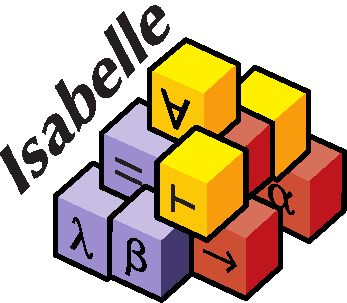
\includegraphics[scale=0.3]{isabelle.pdf}}

\begin{document}

\maketitle

\begin{frame}{This Talk}
  \begin{itemize}
  \item Probabilistic programs (pGCL) + expected running time.\\\pause
     \textbf{Kaminski, Katoen, Matheja, and Olmedo [ESOP 2016]\pause~\textcolor{Gold}{\faStar}}\pause
  \item Two semantics:\pause
  \begin{description}
    \item[Denotational:] \I{\t{pgcl}{\st} \t{=>} \expect \t{=>} \expect} \pause
    \item[Operational:] \I{\big(\t{pgcl}{\st} \times \st\big) \t{=>}
        \t{measure}{\t{stream}{\big(\t{pgcl}{\st} \times \st\big)}}} \pause
    \item[Correspondence:] Denotational $\Leftrightarrow$ Operational \pause
  \end{description}
  \item Examples:\pause
  \begin{itemize}
    \item Simple Random Walk~\textcolor{Crimson}{\faBolt} \pause
    \item Coupon Collector
  \end{itemize}
  \end{itemize}

\begin{center}
  clarified semantics \pause -- different proofs \pause -- fixed proofs
\end{center}
\end{frame}

\begin{frame}{Probabilistic Guarded Command Language (pGCL)}

\[ \I{ \begin{array}{lcl@{\qquad}l}
\t{pgcl}{\st}
& = & \Empty \pause~~|~~ \Skip\pause ~~|~~ \Halt \\
\pause 
& | & \var{x} :\sim \mathcal{D} ~~~\text{or}~~~ \var{x} := \mathsf{expr} & "\c{Assign}~(\st\t{=>}\t{pmf}{\st})" \\
\pause 
& | & \var{p_1}~;\,\var{p_2} \\
\pause 
& | & \var{p_1}~|\,\var{p_2} \\
\pause 
& | & \mathsf{ITE}~\var{g}~\var{p_1}~\var{p_2} &
  \var{g} \hastype  \st \t{=>} \t{bool} \\
\pause 
& | & \mathsf{WHILE}~\var{g}~\mathsf{DO}~\var{p}
\end{array} } \]

\end{frame}

\begin{frame}{Denotational Semantics (Expected Running Time)}
\begin{center}
\I{ \begin{array}{lccl}
\multicolumn{4}{l}{%
\ert \hastype \t{pgcl}{\st} \t{=>}
  (\st \t{=>}{\tikz[overlay] \node[yshift=-0.2ex, xshift=-1.5ex] (post) {};} \t{ennreal}) \t{=>}
  (\st \t{=>}{\tikz[overlay] \node[yshift=1ex, xshift=-1.5ex] (pre) {};} \t{ennreal})} \\[1ex]
\pause
\onslide<2,3>{%
  \begin{tikzpicture}[overlay, shift=(current page.center), yshift=1.5cm, xshift=-2cm]
    \node[fill=cyan!29, rectangle callout, rounded corners, callout absolute pointer=(post)] at (0, 0)
         { Values we want assigned to a \emph{terminal state} } ;
  \end{tikzpicture}%
}%
\pause 
\onslide<3>{%
  \begin{tikzpicture}[overlay, shift=(current page.center), yshift=3.5cm]
    \node[fill=cyan!29, rectangle callout, rounded corners, callout absolute pointer=(pre)] at (0, 0)
         { Values computed for the a \emph{starting state} } ;
  \end{tikzpicture}%
}%
\pause
\ert~\Empty & \var{c}
& = & \var{c} \\[1ex] \pause
\ert~\Skip & \var{c}
& = & 1 + \var{c} \\[1ex] \pause
\ert~\Halt & \var{c}
& = &  0 \\ \pause
\ert~(\c{Assign}~\var{u}) & \var{c}
& = & 1 + \displaystyle \left(\lambda \var{x}.\, \int_{\var{y}} \var{c}~\var{y} ~d(\var{u}\,\var{x})\right) \\[1ex]
\pause
\ert~(\var{p_1};~\var{p_2}) & \var{c}
& = & \ert~\var{p_1}~(\ert~\var{p_2}~\var{c}) \\[1ex] \pause
\ert~(\var{p_1}~|~\var{p_2}) & \var{c}
& = & \ert~\var{p_1}~\var{c} \sqcup \ert~\var{p_2}~\var{c} \\[1ex] \pause
\ert~(\mathsf{ITE}~\var{g}~\var{p_1}~\var{p_2}) & \var{c}
& = & 1 + \big(\lambda \var{x}.\, \c{if} \var{g}~\var{x}
  \c{then} \ert~\var{p_1}~\var{c}~\var{x} \c{else} \ert~\var{p_2}~\var{c}~\var{x}\big) \\[1ex] \pause
\ert~(\mathsf{WHILE}~\var{g}~\mathsf{DO}~\var{p}) & \var{c}
& = & \c{lfp}~\big(\lambda \var{W}\,\var{x}.\, 1~+ \c{if} \var{g}~\var{x}
  \c{then} \ert~\var{p}~\var{W}\,\var{x} \c{else} \var{c}~\var{x}\big)
\end{array} }
\end{center}
\end{frame}

\begin{frame}{Interjection: Markov decision processes}
  \begin{center}\bf Automata with probabilistic and non-deterministic choice\end{center}
  \[ \I{K \hastype \st \t{=>} \t{set}{\t{pmf}{\st}} \quad \quad K\,\stateS \not= \emptyset } \] 
\begin{tikzpicture}[line width=1pt, shorten >=2pt]
  \path [use as bounding box] (-4, -2) rectangle (4, 2) ;
  \alert<8>{\node [draw, circle] (trg) at (3, 0) { $\state{t_1}$ } ;}
\only<2->{ \alert<8>{
  \node [draw, circle] (trg2) at (3, 1) { $\state{t_2}$ } ;
  \node [draw, circle] (trg3) at (3, -1) { $\state{t_3}$ } ;
} }

\only<1-2>{
  \node [draw, circle] (src) at (-3, 0) { $\stateS$ } ;
  \path [->] (src) edge [below] node {\only<2->{$p$}} (trg) ;
  \only<2>{
    \path [->] (src) edge [below] node {\only<2->{$q$}} (trg2) ;
    \path [->] (src) edge [below] node {\only<2->{$r$}} (trg3) ;
  }
}

\only<3->{
  \alert<5>{\node [draw, circle] (src) at (-3, 0) { $\stateS$ } ;}
  \alert<6>{\node [fill, circle, inner sep=2.5pt] (dst) at (0, 0) { } ;
  \node [fill, circle, inner sep=2.5pt] (dst2) at (0, 1) { } ;}

  \path [->] (src) edge [below] (dst) ;
  \path [->] (src) edge [above] (dst2) ;
\alert<7>{
  \path [->] (dst) edge [above right] node {$p$} (trg) ;
  \path [->] (dst) edge [above] node {$q$} (trg2) ;
  \path [->] (dst) edge [below] node {$r$} (trg3) ; }

  \draw[gray!50] (dst2) -- (1.5, 1.25) ;
  \draw[gray!50] (dst2) -- (1.5, 1.75) ;
  \draw[gray!50] (dst2) -- (1, 1.75) ;
}
\end{tikzpicture}

\onslide<4->{
\begin{center}
  Construct maximal expectation $\I{\hat{\mathbb{E}}_{\stateS}[\funF]}$ of a (cost) function $\funF$:
  \[ \I{
      \alert<5>{\hat{\mathbb{E}}_{\stateS}[\funF]} =
      \alert<6>{\bigsqcup_{D \in K~\stateS}}
      \alert<7>{\int_{\state{t}}}
      \alert<8>{~~\hat{\mathbb{E}}_{\state{t}}[\lambda \stateW.~\funF~(\state{t}\cdot\stateW)] ~~}
      \alert<7>{\mathsf{d}D}
    } \]
\end{center}}
\end{frame}

\begin{frame}{Operational Semantics}
\I{ \begin{array}{l@{~}c@{~}c@{~}l}
\multicolumn{4}{l}{%
\K \hastype (\t{pgcl}{\st} \t{*} \st) \t{=>} \t{set}{\t{pmf}{(\t{pgcl}{\st} \t{*} \st)}}} \\[1ex]
\onslide<2->{
\K (\Empty,&\stateS) & = &
\c{det}{\Empty}{\stateS} \\[1ex]
\K (\Skip,&\stateS) & = &
\c{det}{\Empty}{\stateS} \\[1ex]
\K (\Halt,&\stateS) & = &
\c{det}{\Halt}{\stateS} \\[1ex]
}
\onslide<3->{
\K (\c{Assign}~\var{u},&\stateS) & = &
\Big[\lambda \state{s'}.~(\Empty, \state{s'})\Big]~\big\{\var{u}~\stateS\big\} \\[1ex]
}
\onslide<4->{
\K (\var{p_1}~|~\var{p_2},&\stateS) & = & 
\c{det}{\var{p_1}}{\stateS} \cup \c{det}{\var{p_2}}{\stateS} \\[1ex]
}
\onslide<5->{
\K (\mathsf{ITE}~\var{g}~\var{p_1}~\var{p_2},&\stateS) & = &
\c{if} \var{g}\, \stateS \c{then}~ \c{det}{\var{p_1}}{s} ~\c{else}~ \c{det}{\var{p_2}}{\stateS} \\[1ex]
\K (\mathsf{WHILE}~\var{g}~\mathsf{DO}~\var{p},&\stateS) & = &
\c{if} \var{g}\,\stateS \c{then}~ \c{det}{\var{p};~\mathsf{WHILE}~\var{g}~\mathsf{DO}~\var{p}}{\stateS} ~\c{else}~ \c{det}{\Empty}{\stateS} \\[1ex]
}
\onslide<6->{
\K (\var{p_1};~\var{p_2},&\stateS) & = & \left[\lambda%
\begin{array}{ll}
(\Empty, \state{s'}). & (\var{p_2}, \state{s'}) \\
(\Halt, \state{s'}). & (\Halt, \state{s'}) \\
(\var{p'}, \state{s'}). & (\var{p'};~\var{p_2}, \state{s'})
\end{array} %
\right]~\K(\var{p_1}, \stateS)\
}
\end{array} }

\begin{tikzpicture}[overlay, shift=(current page.center), xshift=-5cm, yshift=2.5cm]
\onslide<7>{
  \fill[cyan!20, rounded corners] (-1, 0.4) rectangle (11,-3.4) ;
 
  \node[draw, rounded corners] (P1) at (8, 0) {\I{(\var{x} := 1 | \Halt, \stateS)}} ;
  \node[draw, rounded corners] (P2) at (7, -1) {\I{(\var{x} := 1, \stateS)}} ;
  \node[draw, rounded corners] (P3) at (10, -1) {\I{(\Halt, \stateS)}} ;
  \node[draw, rounded corners] (P4) at (7, -2) {\I{(\Empty, \state{s'})}} ;

  \path[->, >=latex]
    (P1)  edge [bend right=15] (P2)
          edge [bend left=15]  (P3)
    (P3)  edge [in=-90, out=-110, loop] (P3)
    (P2)  edge (P4)
    (P4)  edge [in=-90, out=-110, loop] (P4) ;

  \node (arr) at (5.5, -1) {\I{\stackrel{\Longleftarrow}{\c{DUMMY};\alert{p_2}}}};

  \node[draw, rounded corners] (S1) at (2, 0) {\I{((\var{x} := 1 | \Halt);\alert{p_2}, \stateS)}} ;
  \node[draw, rounded corners] (S2) at (1, -1) {\I{(\var{x} := 1;\alert{p_2}, \stateS)}} ;
  \node[draw, rounded corners] (S3) at (4, -1) {\I{(\Halt, \stateS)}} ;
  \node[draw, rounded corners] (S4) at (1, -2) {\I{(\alert{p_2}, \state{s'})}} ;

  \path[->, >=latex]
    (S1)  edge [bend right=15] (S2)
          edge [bend left=15]  (S3)
    (S3)  edge [in=-90, out=-110, loop] (S3)
    (S2)  edge (S4);
}
\end{tikzpicture}

\end{frame}

\begin{frame}{Traces}
\begin{center}
\begin{tikzpicture}
 
  \node at (0, 6) { Trace } ;
  \node at (5, 6) { \I{\coststream} } ;

  \node[draw, rounded corners] (P1) at (0, 5) {\I{((\var{x} := 1 | \Halt); \var{y} := 0, \stateS)}} ;
  \node (C1) at (5, 5) {\I{0}} ;

\pause

  \node[draw, rounded corners] (P2) at (0, 4) {\I{(\var{x} := 1; \var{y} := 0, \stateS)}} ;
  \path[->, >=latex, double]
    (P1) edge[double] (P2) ;

  \node (p1) at (5, 4.5) {\I{+}} ;
  \node (C2) at (5, 4) {\I{1}} ;

\pause

  \node[draw, rounded corners] (P3) at (0, 3) {\I{(\var{y} := 0, \state{s'})}} ;
  \path[->, >=latex, double]
    (P2) edge[double] (P3) ;

  \node (p2) at (5, 3.5) {\I{+}} ;
  \node (C3) at (5, 3) {\I{1}} ;

\pause

  \node[draw, rounded corners] (P4) at (0, 2) {\I{(\Empty, \state{s''})}} ;
  \path[->, >=latex, double]
    (P3) edge[double] (P4) ;
  \node (p3) at (5, 2.5) {\I{+}} ;
  \node (C4) at (5, 2) {\I{\funF~\state{s''}}} ;

  \node (Pi) at (0, 1.5) {$\vdots$} ;

\end{tikzpicture}
\end{center}

Cost per stream:
\[ \I{
    \coststream~\funF~(\stateS{\cdot}\var{\omega}) \stackrel{\c{lfp}}{=}
    \cost~\funF~\stateS~(\coststream~\funF~\var{\omega})
  } \]
\end{frame}

\begin{frame}{Interjection: Least Fixed Points}
  \begin{theorem}[Transfer rule for least fixed points]
    \[
      \inferrule%
      { \I{\c{supcontinuous}~\funalpha, \funF, \funG} \\
        \I{\funalpha~\bot = \bot} \and \I{\funalpha \circ \funF = \funG \circ \funalpha}}%
      {\I{\funalpha{\tikz[overlay] \node[yshift=-0.2ex, xshift=-1ex] (alpha) {};}
          (\c{lfp}~\funF) ={\tikz[overlay] \node[yshift=-0.2ex, xshift=-1ex] (eq3) {};} \c{lfp}~\funG }}
    \]
  \end{theorem}
\onslide<2>{%
  \begin{tikzpicture}[remember picture, overlay, shift=(current page.center), yshift=-3cm]
    \node[fill=cyan!20, rectangle callout, rounded corners, callout absolute pointer=(eq3)] at (0, 0)
         { \I{\begin{array}{lcl}
             \funalpha (\c{lfp}~\funF) & = &
             \funalpha \circ \funF \circ \funF \circ \funF \circ \funF \circ  \funF \circ \dots \circ \bot \\
             & = & \funG \circ \funG \circ \funG \circ \funalpha \circ \funF \circ  \funF \circ \dots \circ \bot \\
             & = & \funG \circ \funG \circ \funG \circ \funG \circ \funG \circ \dots \circ \funalpha~\bot \\
             & = & \c{lfp}~\funG
           \end{array}}
         } ;
  \end{tikzpicture} }
\onslide<3>{%
  \begin{tikzpicture}[remember picture, overlay, shift=(current page.center), yshift=-3cm]
    \node[fill=cyan!20, rectangle callout, rounded corners, callout absolute pointer=(alpha)] at (0, 0)
         { \I{\displaystyle \funalpha~\funF = \hat{\mathbb{E}}_{\stateS}[\funF]}
           \qquad for $\funF$ Borel-measurable } ;
  \end{tikzpicture} }
\onslide<4>{
  \[ \I{\hat{\mathbb{E}}_{(\var{p}, \stateS)}[\coststream~\funF] =
      \c{lfp}~\left(\bigsqcup_{K~s}~~\int~~\c{cost}\right)}~\var{p}~\stateS \]
}
  
\end{frame}

\begin{frame}{Correspondence Proof}
  \begin{theorem}
    \[ \I{\hat{\mathbb{E}}_{(\var{p}, \stateS)}[\coststream~\funF] = \ert~\var{p}~\funF~\stateS } \]
  \end{theorem}
\pause
  \begin{proof}[Proof by induction on $\var{p}$:]
\pause
  \begin{description}[\I{\mathsf{WHILE}~\var{g}~\mathsf{DO}~\var{p_1}}]
  \item[\I{\var{p_1}; \var{p_2}}] -- Antisymmetry then fixed point induction \\
    \I{\hat{\mathbb{E}}_{(\var{p_1}, \stateS)}[\coststream~(
      \hat{\mathbb{E}}_{(\var{p_2}, {\cdot})}[\coststream~\funF])] =
      \hat{\mathbb{E}}_{(\var{p_1};\var{p_2}, \stateS)}[\coststream~\funF]}
\pause
  \item[\I{\mathsf{WHILE}~\var{g}~\mathsf{DO}~\var{p_1}}] -- Fixed point massaging
\pause
  \end{description}
  \end{proof}

  \begin{itemize}
  \item Operational semantics \& Correspondence $\sim 330$ lines of theory
\pause
  \item Central to our proof: Expectation as fixed point
\pause
  \item \textbf{[KKMO 2016]}: Expectation as sums over all paths
  \end{itemize}
  
\end{frame}

\begin{frame}{Simple Symmetric Random Walk (ssrw)}

\begin{tikzpicture}[state/.style={circle, draw, minimum size=0.75cm, inner sep=0cm}]
  \node[state] (z)  at ( 0, 0) {\small $0$} ;
  \node[state] (p1) at ( 1, 0) {\small $1$} ;
  \node[state] (m1) at (-1, 0) {\small $-1$} ;
  \node[state] (p2) at ( 2, 0) {\small $2$} ;
  \node[state] (m2) at (-2, 0) {\small $-2$} ;
  \node[state] (p3) at ( 3, 0) {\small $3$} ;
  \node[state] (m3) at (-3, 0) {\small $-3$} ;
  \node (pi) at ( 4.5, 0) {$\cdots$} ;
  \node (mi) at (-4.5, 0) {$\cdots$} ;

  \path[->]
    (z)  edge[bend left=30] node[above] {\tiny $1/2$} (p1) 
    (p1) edge[bend left=30] node[below] {\tiny $1/2$} (z)
    (p1) edge[bend left=30] node[above] {\tiny $1/2$} (p2)
    (p2) edge[bend left=30] node[below] {\tiny $1/2$} (p1)
    (p2) edge[bend left=30] node[above] {\tiny $1/2$} (p3)
    (p3) edge[bend left=30] node[below] {\tiny $1/2$} (p2)
    (p3) edge[bend left=30] node[above] {\tiny $1/2$} (pi)
    (pi) edge[bend left=30] node[below] {\tiny $1/2$} (p3) ;

  \path[->]
    (z)  edge[bend left=30] node[below] {\tiny $1/2$} (m1) 
    (m1) edge[bend left=30] node[above] {\tiny $1/2$} (z)
    (m1) edge[bend left=30] node[below] {\tiny $1/2$} (m2)
    (m2) edge[bend left=30] node[above] {\tiny $1/2$} (m1)
    (m2) edge[bend left=30] node[below] {\tiny $1/2$} (m3)
    (m3) edge[bend left=30] node[above] {\tiny $1/2$} (m2)
    (m3) edge[bend left=30] node[below] {\tiny $1/2$} (mi)
    (mi) edge[bend left=30] node[above] {\tiny $1/2$} (m3) ;

\end{tikzpicture}

\begin{itemize}
  \item \I{\Pr_{\var{i}}(\lozenge \var{j}) = 1}
  \item \I{H~\var{i}~\var{j} := \ert~(\mathsf{ssrw}~\var{j})~\bot~\var{i}} \\
    for \I{\var{i} \not= \var{j}}: \I{H~\var{i}~\var{j}= \pause \infty}
\end{itemize}
\end{frame}

\begin{frame}{Simple Symmetric Random Walk -- [KKMO]}
  \begin{center}
    How do \textbf{Kaminski, Katoen, Matheja, and Olmedo} prove it?
  \end{center}
  \begin{itemize}
  \item<2-> \I{\ert~(\mathsf{ssrw}~\var{j})~\bot~\var{i}} has lower $\omega$-invariant
    \I{I_{\var{n} + 1} \le \ert~\mathsf{STEP}~I_{\var{n}} }:
    \[ \I{I_{\var{n}} = 1 + \llbracket 0 < \var{x} \le \var{n} \rrbracket \cdot \infty} \]
  \item<3-> They need to prove this equation: \\
    \I{1 + \llbracket \var{x} > 0 \rrbracket \cdot 2 +
      \llbracket 1 < \var{x} \le \var{n} + 1 \rrbracket \cdot \infty +
      \llbracket 0 < \var{x} \le \var{n} - 1 \rrbracket \cdot \infty =} \\
    \I{1 + \llbracket \var{x} > 0 \rrbracket \cdot 2 + \llbracket 0 < \var{x} \le
      \var{n} + 1 \rrbracket \cdot \infty}
  \onslide<4>{
  \begin{tikzpicture}[overlay, shift=(current page.center), yshift=-2cm]
    \node [draw=red, rotate = 45, scale = 3, text = red, rounded corners, line width = 4pt] at (0, 0) { ERROR };
  \end{tikzpicture} }
  \onslide<5>{
  \begin{tikzpicture}[overlay, shift=(current page.center), yshift=-3.2cm]
    \node[fill=red!29, rounded corners, inner sep=5mm] at (0, 0) {\parbox{7cm}{
        Fails for \I{\var{x} = 1} and \I{\var{n} = 0}.
    }};
  \end{tikzpicture} }
  \end{itemize}
\end{frame}

\begin{frame}{Simple Symmetric Random Walk -- our Solution}
  Use \I{H~\var{i}~\var{j} = \hat{\mathbb{E}}_{(\mathsf{ssrw}~\var{j}, \var{i})}[\coststream{\tikz[overlay] \node[yshift=0.4ex, xshift=-4ex] (post) {};}]} to prove
  \[ \I{H~\var{i}~\var{j} = H~\var{i}~\var{k} + H~\var{k}~\var{j}} \quad \text{for} \quad \I{\var{i} \le \var{k} \le \var{j}} \]

  \begin{tikzpicture}[overlay, shift=(current page.center), yshift=2cm, xshift=-2cm]
    \node[fill=cyan!29, rectangle callout, rounded corners, callout absolute pointer=(post)] at (0, 0)
         { Operational semantics -- trace representation } ;
  \end{tikzpicture}%

\pause
  Then derive \I{H~\var{i}~\var{j} = \infty} for \I{\var{i} \not= \var{j}}
  \pause \textcolor{green}{\Large \checkmark}
\end{frame}


\begin{frame}{Coupon Collector}
\[\I{
\begin{array}{lcl}
\var{x} := 0, \var{i} := 0, \var{cp} := [\overbrace{F, \ldots, F}^{\var{N}~\textrm{times}}]; &
&
\onslide<2->{\var{c} := 0, \var{b} := F;}
\\
\mathsf{WHILE}~\var{x} < \var{N}~\mathsf{DO} &
\onslide<3->{\var{x} \rightarrow \var{c}} &
\onslide<2->{\mathsf{WHILE}~\var{c} < \var{N}~\mathsf{DO}}
\\
\quad \mathsf{WHILE}~\var{cp}[\var{i}]~\mathsf{DO} &
\quad \onslide<3->{\var{cp}[\var{i}] \rightarrow \var{b}} \quad &
\onslide<2->{\quad \mathsf{WHILE}~\var{b}~\mathsf{DO}}
\\
\quad \quad \var{i} :\sim \mathcal{U}(\{1, \ldots, \var{N}\}); &
\onslide<3->{|\var{cp}| = \var{x}} &
\onslide<2->{\quad \quad \var{b} :\sim \mathcal{B}(\var{x}/\var{N});}
\\
\quad \var{cp}[\var{i}] := T, \var{x} := \var{x} + 1 &
&
\onslide<2->{\quad \var{b} := T, \var{c} := \var{c} + 1}
\end{array}}
\]

\I{\ert~\mathtt{CC}_{\var{N}}~0~\stateS =
  2 + \var{N}\cdot\left(4 + 2\sum_{\var{i} = 1}^{\var{N}} \frac{1}{\var{i}}\right)}.
\begin{center}
\onslide<4->{ \textbf{KKMO} use loop invariants to prove running time }
\end{center}
\end{frame}

\begin{frame}{Related Work}
  Different pGCL formalizations already exist:
\pause
  \begin{description}[Celiku \& McIver~{[N. J. C. 2004]}]
  \item[Hurd~\emph{et~al.}~{[QAPL 2003]}] VCG in HOL, deep
\pause
  \item[Celiku \& McIver~{[N. J. C. 2004]}] Expected running time 
    \begin{itemize}
    \item Allow cost analysis for pGCL
    \item Refinement only for upper bounds
    \item No relation to an operational model
    \end{itemize}
\pause
  \item[Cock {[SSV 2012]}] VCG in Isabelle/HOL, shallow
  \end{description}
\end{frame}

\begin{frame}{Conclusion \& Future Work}
  \begin{itemize}
  \item Relating denotational and operational semantics
\pause
  \item Explore use cases where this relation simplifies proofs\\
\pause
    \textbf{Loop invariants are not always enough}
\pause
  \item Explore: Probabilistic relational Hoare logic (pRHL) + non-determinism
  \end{itemize}
\end{frame}

\end{document}
